
%-------------------------------------------------------------% 
\pagebreak
\subsection{Process of Assembly}

\begin{table}[H]
\centering
\renewcommand{\arraystretch}{1.3}
\begin{tabular}{|p{4cm}|p{10cm}|}
\hline
\rowcolor{gray!15}
\textbf{Step} & \textbf{Action / Details} \\
\hline
\rowcolor{gray!5}
\multicolumn{2}{|c|}{\textbf{PCB Bring-Up}} \\
\hline
Unbox PCB & Inspect for solder mask defects, visual solder bridges, and damaged pads. \\
\hline
Continuity Test & 1) VBAT to GND (no short)  \newline 2) 3V3 to GND (no short)  \newline 3) Key nets per schematic. \\
\hline
ESD Protection & Use ESD mat and strap before populating components. \\
\hline
Populate Components & 1) 10 µF capacitor  \newline 2) 100 nF capacitor  \newline 3) ESP32 module  \newline 4) Female header pins: bent pins outwards for front sensor, vertical pins downward for bottom sensor. \\
\hline
Post-Solder Check & Perform continuity test on soldered components. \\
\hline
Voltage Rails & Verify 3V3 = 3.3 V. \\
\hline
Temperature Check & Ensure no component is abnormally hot at idle. \\
\hline
\rowcolor{gray!5}
\multicolumn{2}{|c|}{\textbf{3D-Printed Frame Assembly}} \\
\hline
Print Frame & 1) Material: PETG  \newline 2) Supports: tree  \newline 3) Infill: ~7\% gyroid  \newline 4) Wall thickness: 2 perimeters. \\
\hline
Post-Processing & 1) Remove supports and smooth edges; inspect for defects  \newline 2) Open front of frame for PCB insertion  \newline 3) Ensure no component contacts 3D printed surfaces; PCB sits flush  \newline 4) Slide motors into friction-fit holders. \\
\hline
Check Fit & 1) PCB flat  \newline 2) Connectors accessible  \newline 3) No compression on ESP32  \newline 4) Edges flush. \\
\hline
\rowcolor{gray!5}
\multicolumn{2}{|c|}{\textbf{Modular Options Assembly}} \\
\hline
Battery Cage & 1) Optionally insert under main frame. \\
\hline
Camera Module Holder & 1) Optionally attach on top of main frame. \\
\hline
Leg Pieces & 1) Insert into designated holes under main frame. \\
\hline
\rowcolor{gray!5}
\multicolumn{2}{|c|}{\textbf{Pre-Run Checks}} \\
\hline
Lead Routing & 1) Route motor/JST leads away from rotor sweep  \newline 2) Secure with tie-downs. \\
\hline
Clearance Check & 1) Ensure full clearance with guards  \newline 2) No wire chafe  \newline 3) Connectors latched  \newline 4) Motors held firmly. \\
\hline
Mechanical Tests & 1) Run shake or stability tests \textit{[location TBD]}. \\
\hline
Firmware Test & 1) Power on without propellers  \newline 2) Confirm ESP32 boots, sensors initialise  \newline 3) Each motor spins once  \newline 4) Verify serial output, LED states correct. \\
\hline
\end{tabular}
\caption{ESP Assembly and Pre-Run Procedure}
\label{tab:esp-assembly-numbered}
\end{table}

\textbf{Soldering Guide} \\
The following steps illustrate the initial PCB soldering process, showing component placement and orientation.

\begin{figure}[H]
    \centering
    \begin{subfigure}[b]{0.4\textwidth}
        \centering
        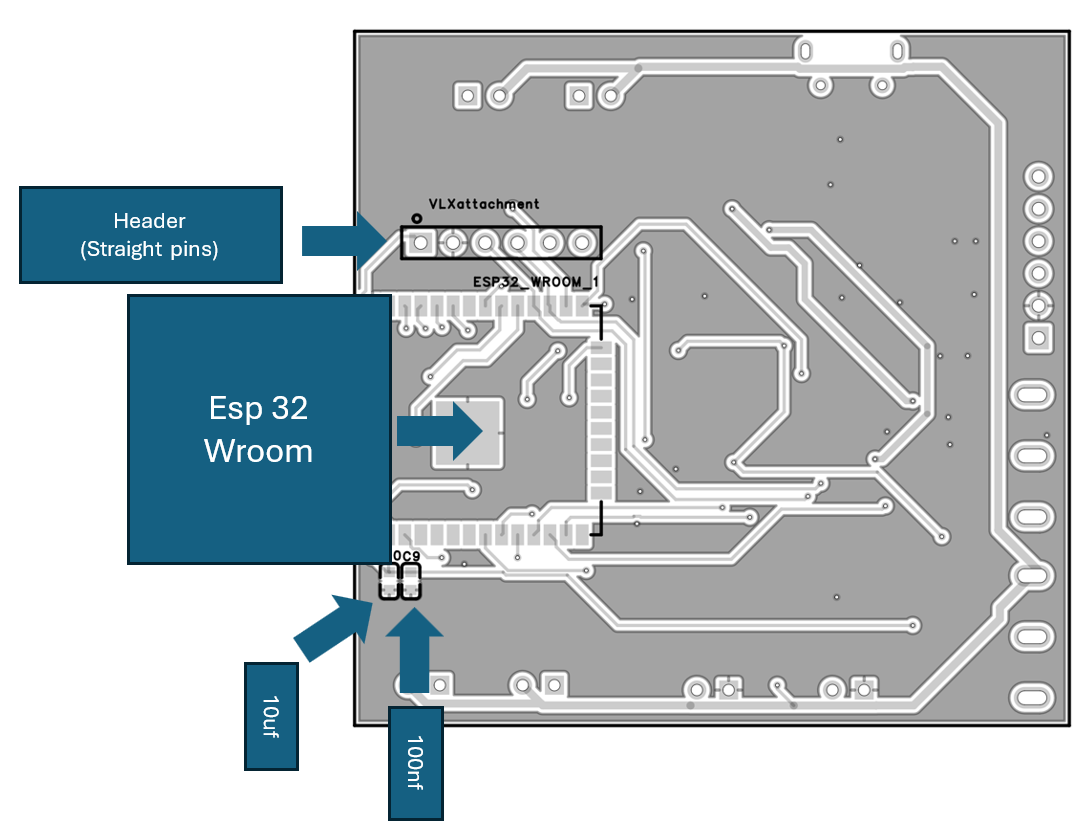
\includegraphics[width=\textwidth]{img/assembly-1.png}
        \caption{Step 1}
    \end{subfigure}
    \hfill
    \begin{subfigure}[b]{0.4\textwidth}
        \centering
        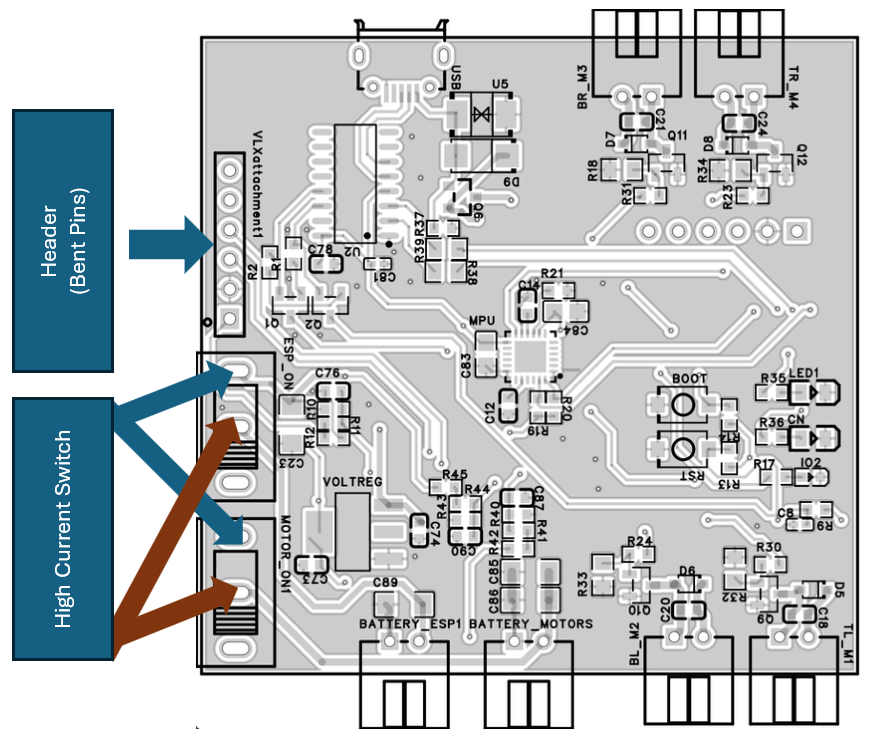
\includegraphics[width=\textwidth]{img/assembly-2.png}
        \caption{Step 2}
    \end{subfigure}
    \caption{ESP Assembly Steps}
\end{figure}

\textbf{Main Frame} \\
This image shows the 3D-printed main frame of the drone, which provides structural support for the PCB, motors, and any modular components.

\begin{figure}[H]
    \centering
    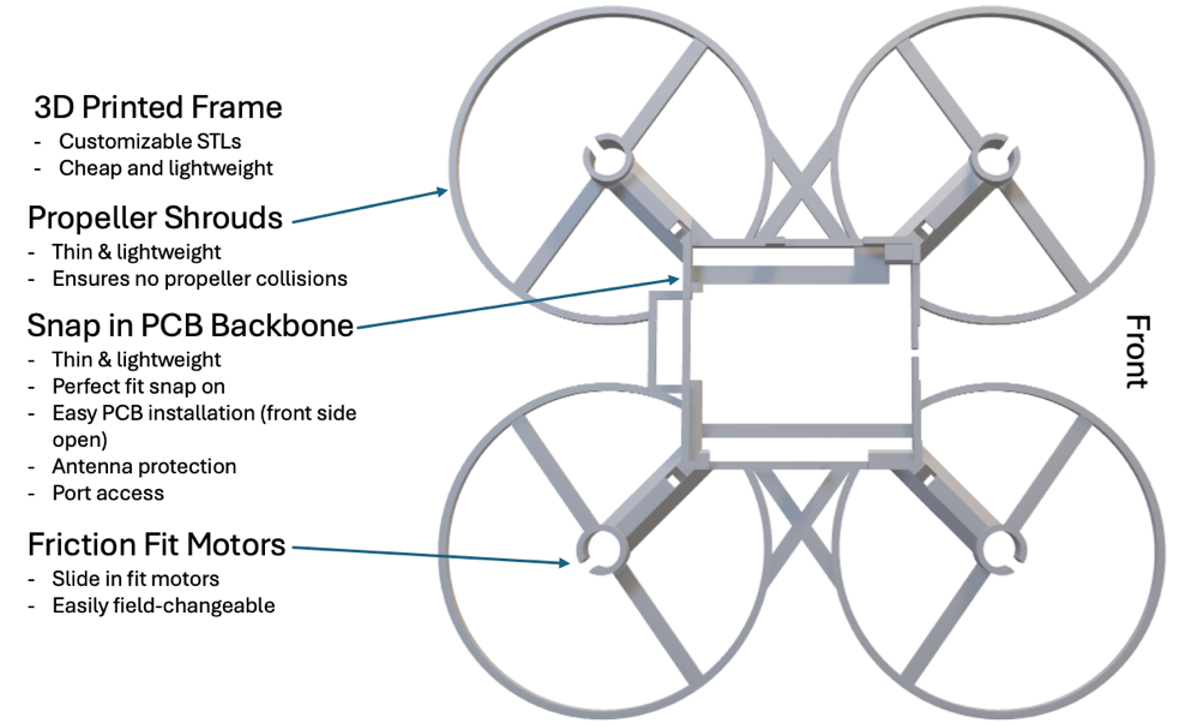
\includegraphics[width=0.8\textwidth]{img/assembly-3.png}
\end{figure}

\pagebreak
\textbf{Frame Additions} \\
These figures illustrate optional components being inserted into the main frame, such as the camera holder and legs and can be removed, changed and altered easily to fit with the main frame.

% \begin{figure}[H]
%     \centering
%     \begin{subfigure}[b]{0.48\textwidth}
%         \centering
%         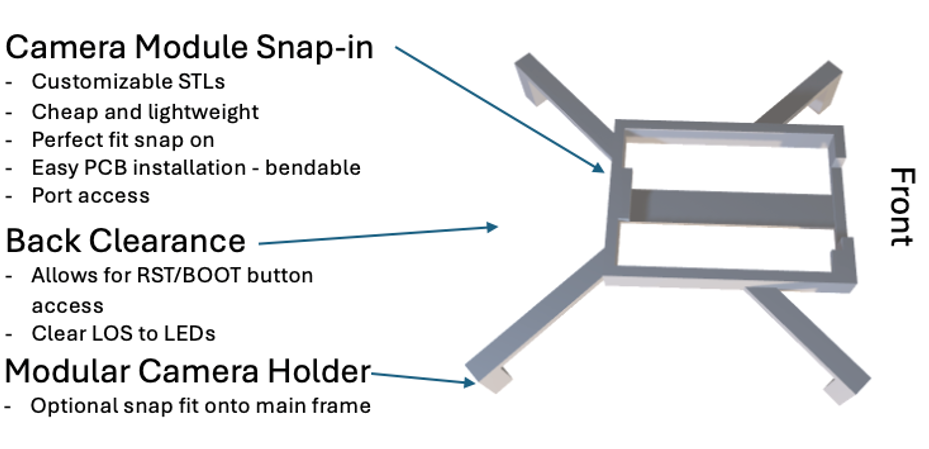
\includegraphics[width=\textwidth]{img/assembly-4.png}
%         \caption{Step 1}
%         \label{fig:assembly-4}
%     \end{subfigure}
%     \hfill
%     \begin{subfigure}[b]{0.48\textwidth}
%         \centering
%         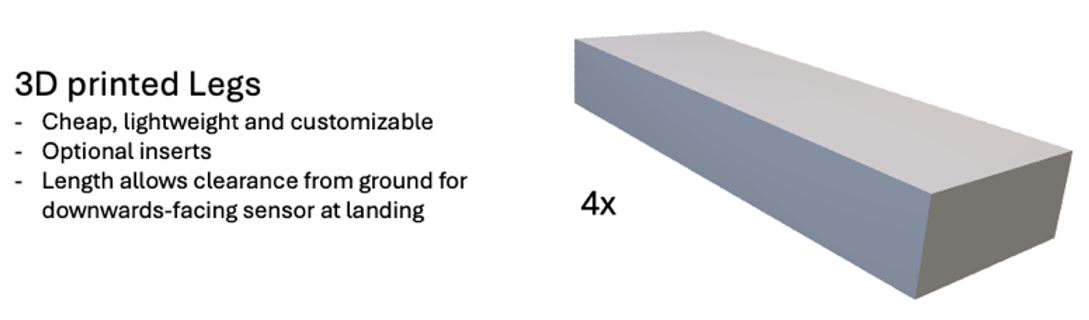
\includegraphics[width=\textwidth]{img/assembly-5.png}
%         \caption{Step 2}
%         \label{fig:assembly-5}
%     \end{subfigure}
%     \caption{ESP Assembly Steps}
%     \label{fig:extras-assembly-steps}
% \end{figure}

\begin{figure}[H]
    \centering
    \begin{subfigure}[b]{0.3\textwidth}
        \centering
        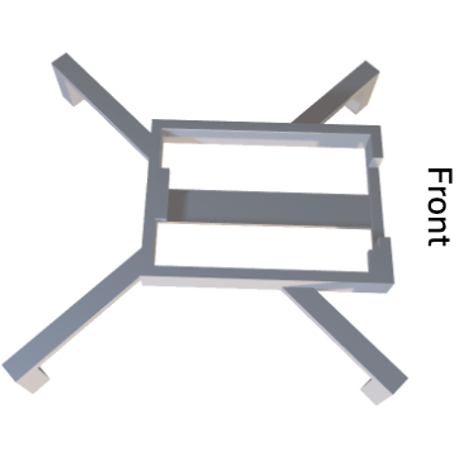
\includegraphics[width=\textwidth]{img/assembly-4b.png}
        \caption{Camera Mount}
    \end{subfigure}
    \vspace{0.5cm}
    \begin{subfigure}[b]{0.3\textwidth}
        \centering
        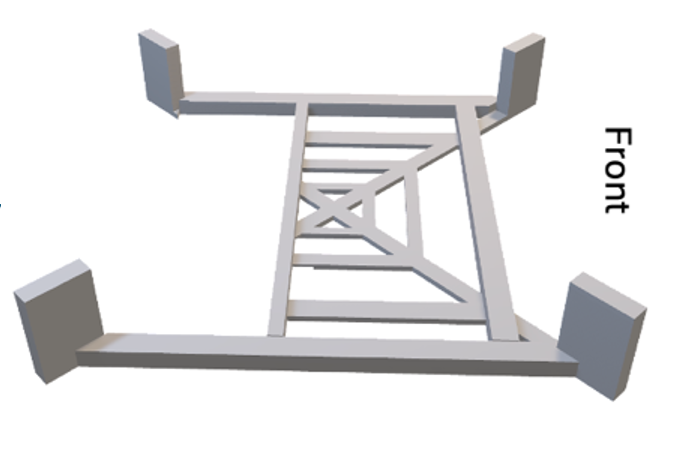
\includegraphics[width=\textwidth]{img/assembly-9b.png}
        \caption{Battery Holder}
    \end{subfigure}
    \vspace{0.5cm} 
    \begin{subfigure}[b]{0.25\textwidth}
        \centering
        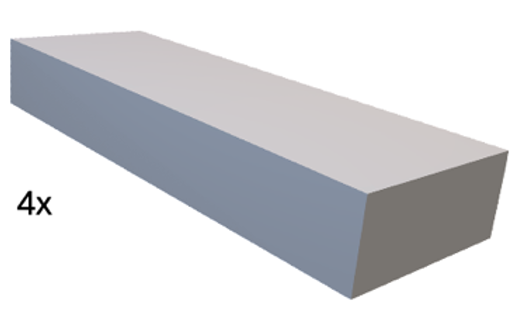
\includegraphics[width=\textwidth]{img/assembly-5b.png}
        \caption{Drone Foot}
    \end{subfigure}
    \caption{Frame Assembly Process}
\end{figure}

% \begin{figure}[H]
%     \centering
%     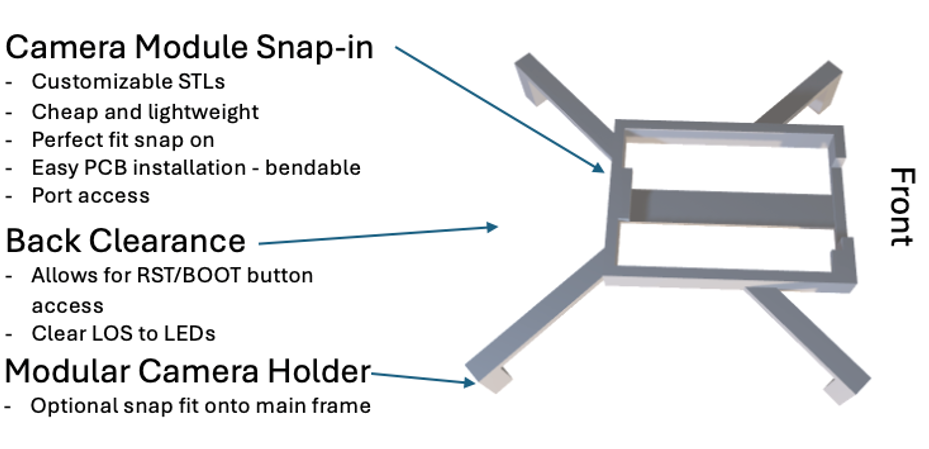
\includegraphics[width=0.6\textwidth]{img/assembly-4.png}
% \end{figure}

% \begin{figure}[H]
%     \centering
%     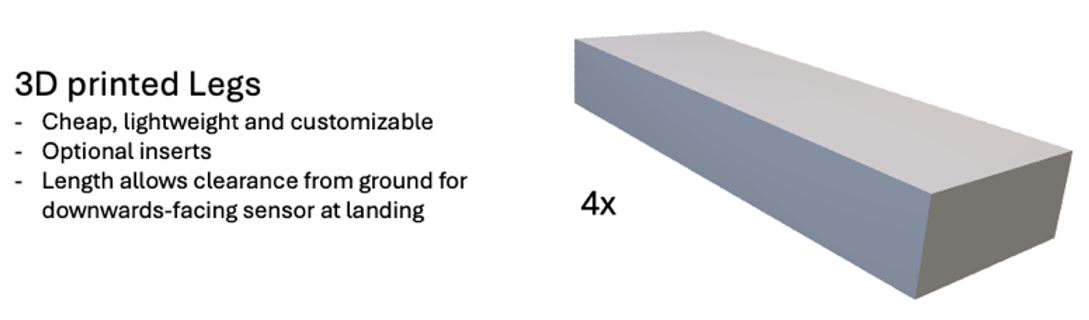
\includegraphics[width=0.6\textwidth]{img/assembly-5.png}
% \end{figure}

% \begin{figure}[H]
%     \centering
%     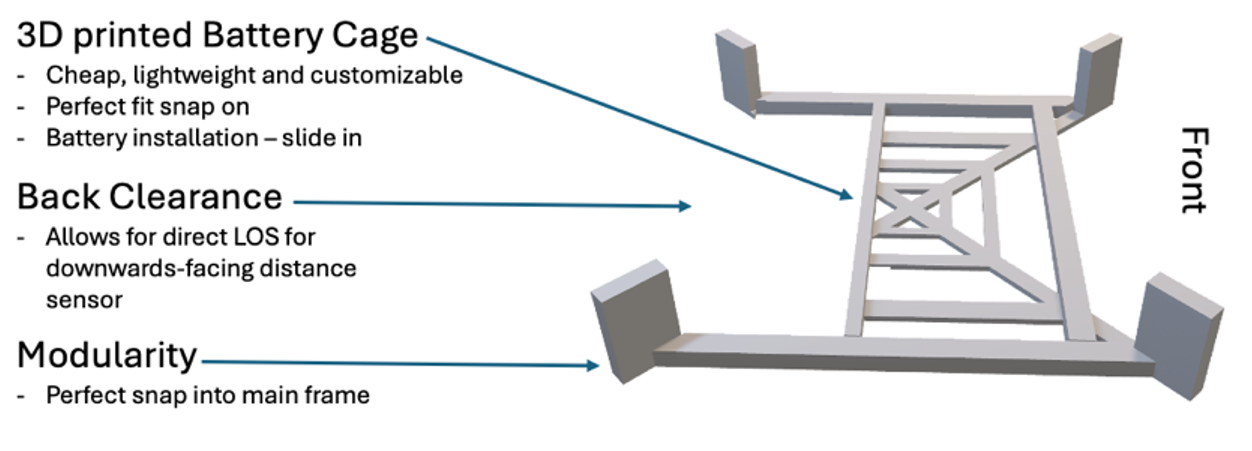
\includegraphics[width=0.6\textwidth]{img/assembly-9.png}
% \end{figure}

% \pagebreak
\textbf{Frame Assembly} \\
The following figures demonstate how the additional frame components can be added to the main frame.

\begin{figure}[H]
    \centering
    \begin{subfigure}[b]{0.45\textwidth}
        \centering
        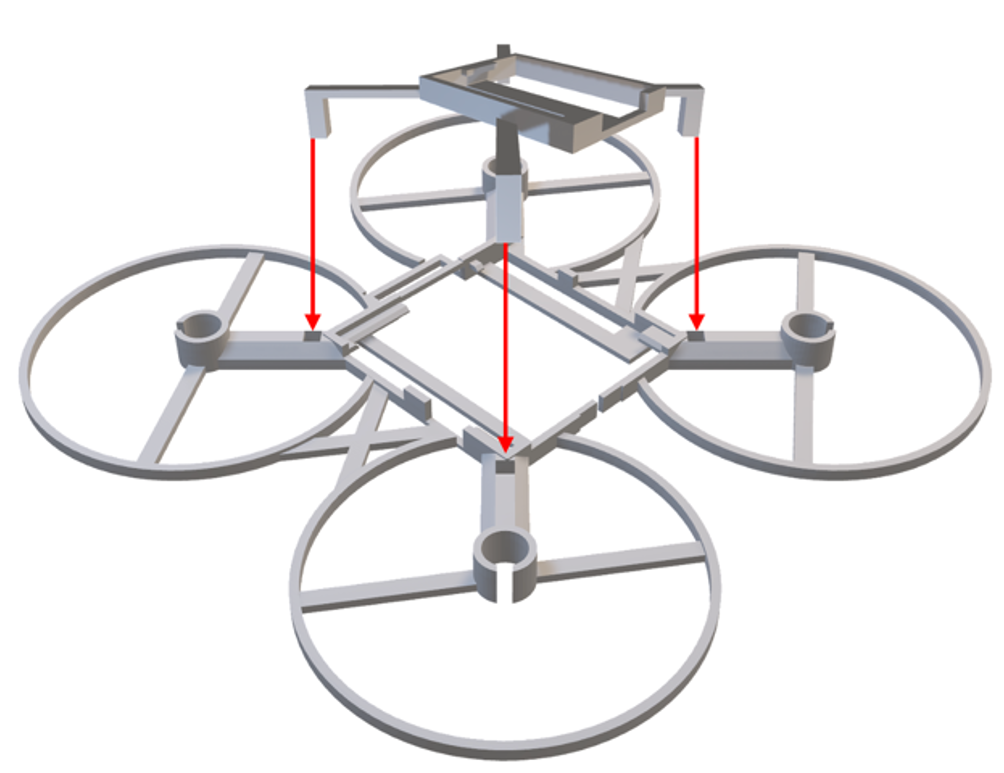
\includegraphics[width=\textwidth]{img/assembly-6.png}
        \caption{Camera Mount}
    \end{subfigure}
    % \vspace{0.5cm} 
    \begin{subfigure}[b]{0.35\textwidth}
        \centering
        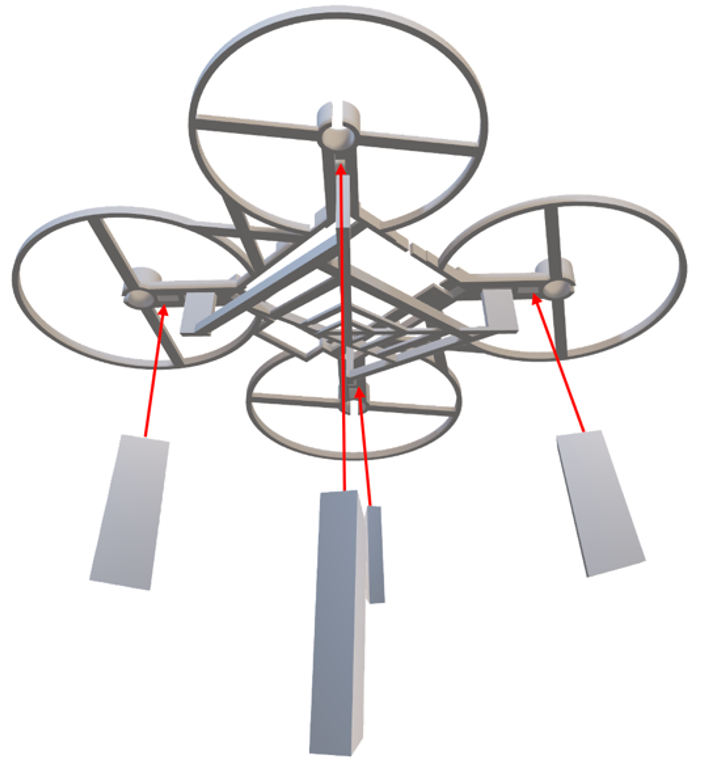
\includegraphics[width=\textwidth]{img/assembly-7.png}
        \caption{Drone Foot}
    \end{subfigure}
    % \vspace{0.5cm}
    \begin{subfigure}[b]{0.35\textwidth}
        \centering
        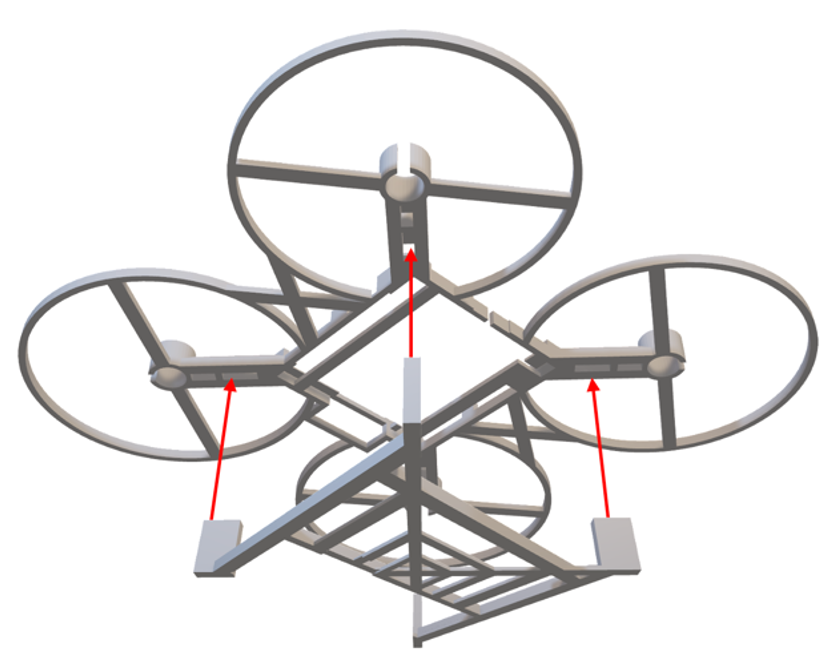
\includegraphics[width=\textwidth]{img/assembly-8.png}
        \caption{Battery Holder}
    \end{subfigure}
    \caption{Frame Assembly Process}
\end{figure}

\pagebreak
A summary of the additions is given below in Table~\ref{tab:frame-add-summary}.

\begin{table}[H]
\centering
\begin{tabular}{|p{3cm}|p{11cm}|}
\hline
\textbf{Module} & \textbf{Features} \\
\hline
Camera Module Snap-In &
o Customizable 3D-printed STL files for design adjustments \newline
o Lightweight and cost-effective \newline
o Perfect snap fit onto main frame \newline
o Easy PCB installation; bendable as needed \newline
o Provides access to ports/connectors \newline
o Back clearance for RST/BOOT buttons and status LEDs \newline
o Optional snap-on camera holder for modularity \\
\hline
3D-Printed Battery Holder & 
o Lightweight, customizable, affordable \newline
o Snap-fit onto main frame \newline
o Easy battery installation \newline
o Back clearance for downward-facing distance sensor \newline
o Supports modular quick insertion/removal \\
\hline
3D-Printed Legs / Drone Feet & 
o Cheap, lightweight, customizable \newline
o Optional inserts for flexible landing configuration \newline
o Sufficient leg length for sensor clearance \newline
o Four legs improve frame stability \\
\hline
\end{tabular}
\caption{Summary of Modular Frame Additions}
\label{tab:frame-add-summary}
\end{table}